\setchapterpreamble[u]{\margintoc}
\chapter{Optimization \& Gradient Descent}
\labch{Optim}

\section{Optimization Problem}
With the foundation of neural networks in computer vision laid out, it seems as if one could easily start off with these right away.
Yet, one very important part is still missing, which is the optimizer.
Every neural network as it has been presented is based on weights which are meant to be trained.
Without training, neural networks are of little use and would basically just generate pseudo-random output.

This is where optimizers come in.
Optimzers have played a very important role for the development of neural networks and their comeback after the so-called 'AI winter'.
The goal of an optimizer, is to find weights such that a neural network fulfills its intended task.
Mathematically this equal to finding a minimum of a loss function which has been introduced in \refsec{ANN}.

The optimizer is defined as an algorithms which searches for weights, which minimize said loss function.
Hence, the network is optimized according to its loss function.

Very early implementations of networks like the perceptron or the McCulloch-Pitts model, had very straight forward algorithms for finding these weights.
As these networks were inspired by nature and so was the optimizer.
In accordance to observations made on neurons, weights were trained according to Hebb's rule~\cite{ommer}.
Simply speaking it says "neurons wire together if they fire together"~\cite{hebb}.
Say, two neurons are in subsequent layers of a network and given some input, they are both activated.
Then Hebb's rule states that the weight that connects them is increased like
\begin{align}
    \Delta w_{ij} & = \eta \cdot a_i \cdot b_j \\
    w_{ij} & \rightarrow w_{ij} + \Delta w_{ij}
\end{align}
for $\Delta w_{ij}$ the weight update, $\vec{a}, \vec{b}$ the activation vectors for the respective layers and $\eta$ the learning rate.
Since the McCulloch-Pitts only knows the states active $a_i = 1$ and inactive $a_i = 0$, this rule will increase the weights between synchronously firing neurons.

The \textbf{learning rate} $\eta$ is an important parameter in many optimizers that decides how large an update step will be.
A learning rate too high will often results in uncontrolled behaviour as the optimizer changes the weights too much and overshoots the optimal point
A too-low learning rate results in slow convergence and thus wasted time.
Also, an optimizer with a low learning rate can more easily get stuck in local minima (more on that later).

Even though the conformity of Hebb's rule with nature has been shown~\cite{lomo}, it is rather obvious that it does not factor in the loss function.
Other approaches have tried to improve Hebb's learning rule and also address problems like instability~\cite{ojas_rule}.
Still, Hebb's rule is clearly not well suited for finding suitable weights.

A slightly more intuitive, yet not inspired by nature, optimization algorithm is the perceptron algorithm.
As the name states, it is used to update a perceptron.

\refsec{ANN} already stated, that the perceptron is equal to a linear classifier.
The perceptron algorithm leverages this analogy and implements a very straight forward optimization algorithm: \\
If the perceptron correctly classifies a point, then do not change anything. 
If a point is wrongly classified, move the decision boundary in direction of the wrongly classified point.\\
This update rule will ideally move the decision boundary repeatedly until the boundary crosses all wrongly classified points.
\begin{align}
    \labeq{perceptron_algo}
    \Delta w_{ij} & = \eta \cdot \frac{1}{2}(\tilde{y}^k_i - y^k_i) \cdot x^k_j \\
    w_{ij} & \rightarrow w_{ij} + \Delta w_{ij}
\end{align}
with $\tilde{\vec{y}}$ the desired activations/classification, $\vec{y}$ the observed classification, $i,j$ the indices for units in each layer.
$\vec{x}^k$ is the input for a sample with index $k$ from the previous layer.
$(\tilde{y}^k_i - y^k_i$ is non-zero only if $\vec{x}^k$ is misclassified and the factor then scales this term to $1$.
The sign of this term will indicate in which direction the decision boundary should move.
The weight update also scales with $x^k_j$ since the amplitude and the sign of the input are important to pick the correct weight.

If the optimization algorithm comes to a stop, since all classifications are correct, then the classification error has been minimized as well.

\section{Gradient Descent}
The idea of the perceptron algorithms can now be generalized further such that it uses the previously defined loss or cost functions (see \refch{MLandCV}).
Instead of updating each neuron at a time, update everything!

Thus, the term $\frac{1}{2}(\tilde{y}^k_i - y^k_i)$ in \refeq{perceptron_algo} must change.
The purpose of this term is that it indicates in which direction the boundary should move.
Now the question is how to determine this direction for an arbitrary loss function $L^k$ that return a scalar score for a given sample $\vec{x}^k$.

By looking at a single weight at a time, the scalar output of the loss function depends on the scalar value of each single weight.
Thus, $L^k$ can be visualized in a 2D graph.
\begin{marginfigure}
    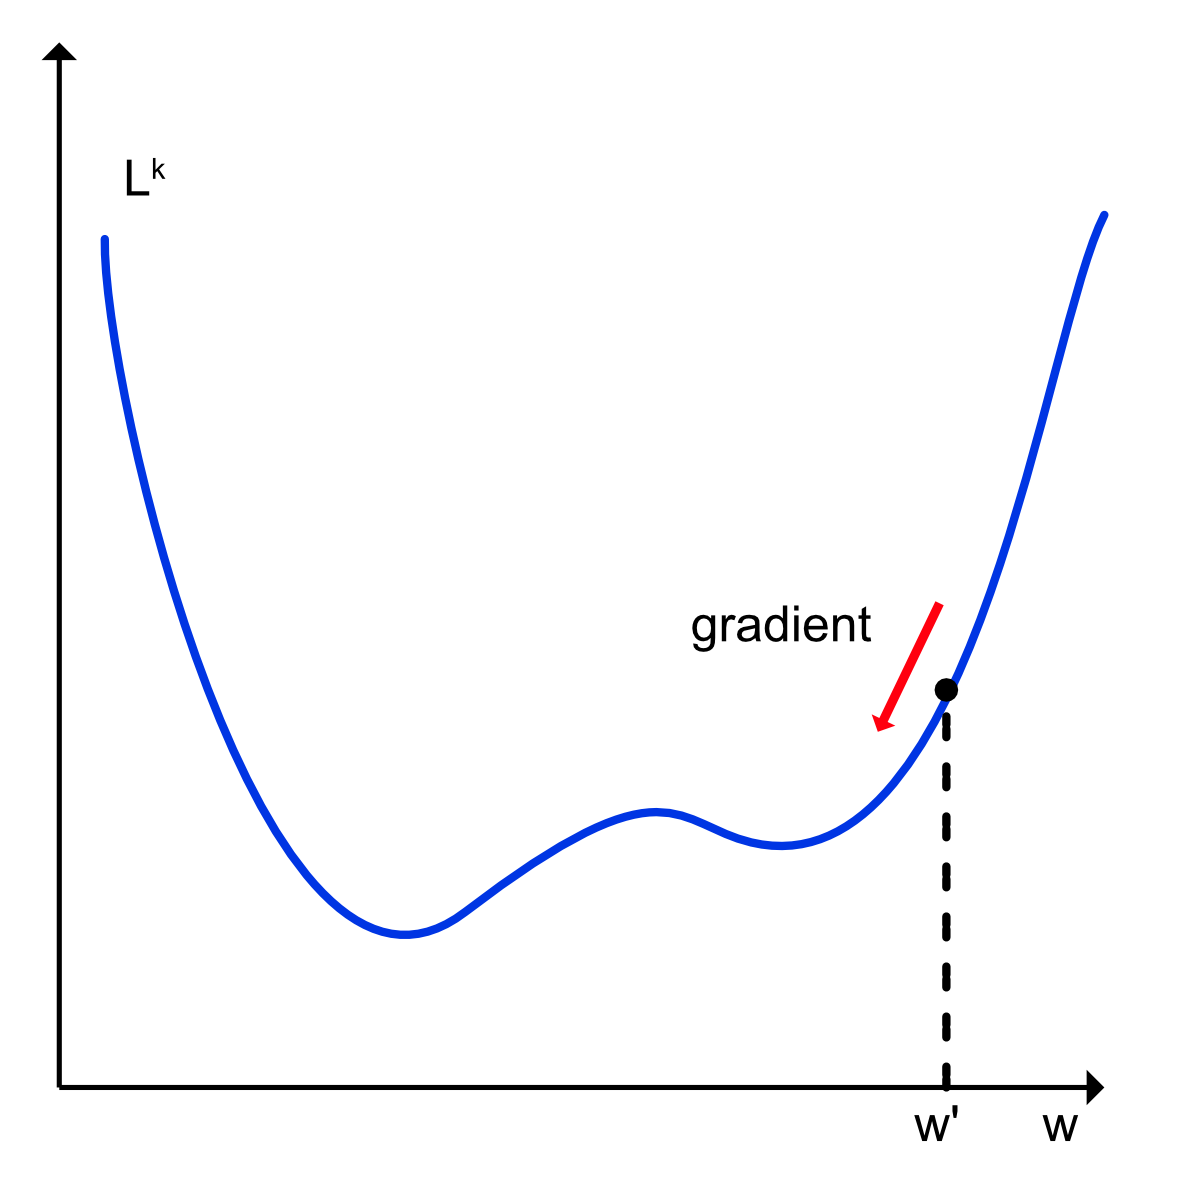
\includegraphics{grad}
    \caption{Example depiction of loss function $L^k$ against $w$. At point $w'$ the slope points the minimum.}
    \labfig{loss_function}
\end{marginfigure}
Looking at such a depiction (see \reffig{loss_function}) the weight should change such that the loss function is minimized.
This can be achieved by following the slope at position $w$, as it points towards the minimum.
The slope in this graph is equivalent to the negative gradient of the function at point $w$, which can be easily calculated, if the dependence between $L(w)$ and $w$ is known.
By taking a small step along the direction the negative gradient points in (see previous section) the loss function becomes smaller but still has likely not reached its minimum.
Thus, the gradient again calculated again for a new $w$ and --again-- $w$ is updated in direction of the gradient.

Applying this procedure iteratively will reduce the loss function in a step-wise manner by descending along the gradient, thus the name \textbf{gradient descent}.

Besides giving information about the direction, the gradient also includes information about the steepness of the slope.
For a continuous loss function $L^k$ the gradient will become smaller the closer the $w$ is to the minimum as $\tilde{w}$.
Consequently, a larger gradient will indicate that a larger update step is possible.\\
The equation for calculating $\Delta w_{ij}$ then becomes:
\begin{align}
    \labeq{gradientrule}
    \Delta w_{ij} & = - \eta \cdot \frac{\partial L^k}{\partial w_{ij}} \cdot x^k_j \\
    w_{ij} & \rightarrow w_{ij} + \Delta w_{ij}
\end{align}
with $\frac{\partial L^k}{\partial w_{ij}}$ the partial derivative of $L^k$ with respect to $w_{ij}$.

The same principle can be applied to many weights at the same time, where each gradient is calculated with respect to the respective weight.
\begin{marginfigure}
    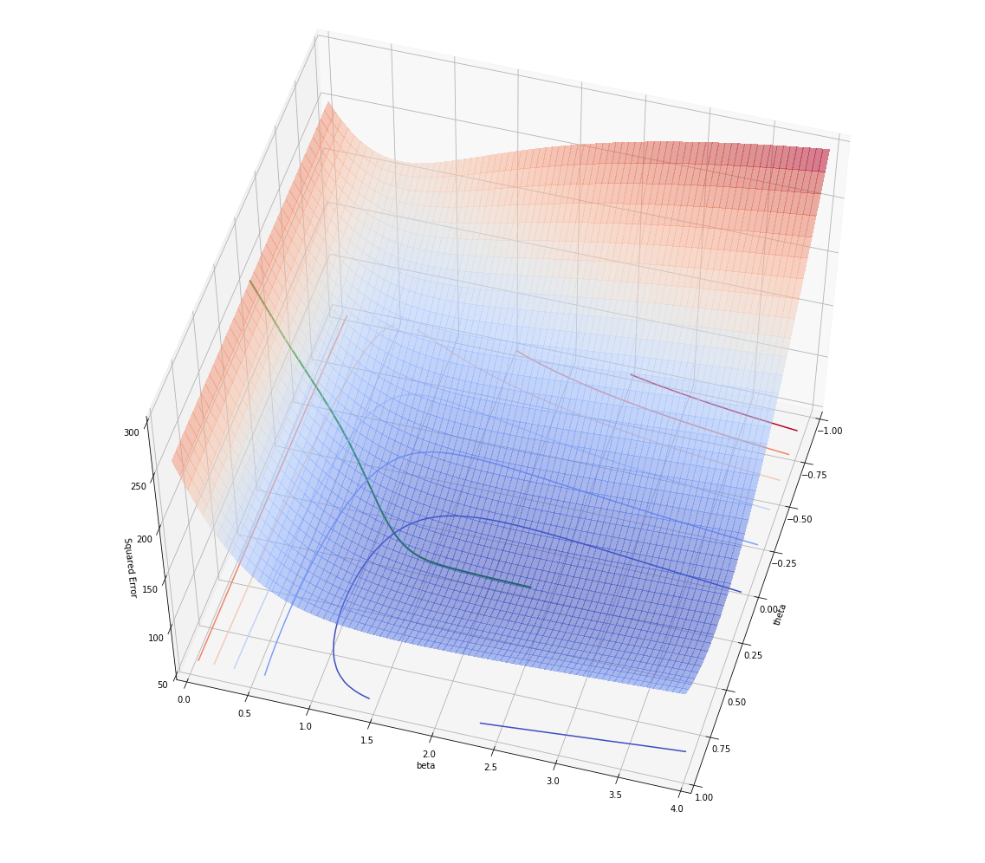
\includegraphics{3Dgrad}
    \caption{3D plot of loss function for two  weights $w_1$ and $w_2$.}
    \labfig{3dloss_function}
\end{marginfigure}
Also, the gradient can easily be evaluated over the whole data set now $k = 1, 2,...$
Thus, \refeq{gradientrule} can be rewritten in vectorized notation:
\begin{align}
    \Delta \mat{w} & = - \eta \cdot \frac{1}{N} \sum_{k=1}^{N} \frac{\partial L^k}{\partial \mat{w}} \cdot \vec{x}^k \\
    \mat{w} & \rightarrow \mat{w} + \Delta \mat{w}
\end{align}

Gradient descent allows to find minima for any loss function as long as the output is differentiable in any weight $w$.
This means that the same principle also applies to deep neural networks.
However, there are two problems left.\\
First, how to obtain the gradient easily (especially for many layers), as analytical differentiation is hard to do for every weight, yet numerical differentiation is very costly~\cite{ommer}.
The answer to this is automatic differentiation with back-propagation, which will be explained in the next section.\\
The second problem is, how to avoid local minima.
One could argue, that local minima would also solve the problem sufficiently and especially for many weights it is unlikely to find the global minimum.
Yet, shallow local minima can still be problematic if the optimizer gets stuck in these.

\subsection{Stochastic Gradient Descent}
Stochastic gradient descent (SGD) is one possible solution for this problem alongside another problem that comes with gradient descent.
For large $N$ it takes very long calculate all gradients and then take the mean.
In comes SGD which does not take the mean over all samples but applies the gradient for each sample.\\
This introduces some randomness into the training as two samples can very quite much (\eg photographs).
As two samples vary in their loss functions, so does the loss hyperplane, and local minima change constantly.
Yet this approach comes with a trade-off since the hyperplane changes so much.
It could prohibit convergence as the changes become too large and there is no common gradient vector along which the optimizer can move.

The solution to this problem is \textbf{mini-batch gradient descent} as an intermediate solution.
Instead of taking the mean over the whole data set, it takes the mean over a mini-batch, which consisting of a smaller number of samples.
Typical choices are in the order of 32 samples per mini-batch plus-minus an order of magnitude.

\subsection{Momentum}
Another solution is adding momentum to SGD.\\
By saving the direction of the previous SGD update and including it into its current step, the 'momentum' from the previous step is carried over \cite{ommer}.
\begin{align}
    \mat{w}_t & = \mat{w}_{t-1} + \Delta \mat{w}_{t-1}
    \Delta \mat{w}_t & = - \eta \cdot \frac{1}{N} \frac{\partial L^k}{\partial \mat{w}_t} \cdot \vec{x}^k + \gamma \Delta \mat{w}_{t-1}
\end{align}

There are notable improvements to this method such as the Nesterov momentum update \cite{ommer}

\subsection{AdaM \& AdaGrad}
\textbf{AdaGrad} takes a different approach in viewing the learning rate $\eta$ as a hyper parameter which is tunes for each weight.
Basically, weights which are updated frequently (often large $\Delta w_{ij}$) should receive smaller updates.
On the other hand rarely updates weights should receive larger updates.
The result is "elementwise scaling of the gradient based on the historical sum of squares in each dim" \cite{ommer}
\begin{align}
    \Delta \mat{w}_t & = - \frac{\eta}{\sqrt{\epsilon \mat{I} + \text{diag}(\mat{G}_t)}} \cdot \frac{1}{N} \frac{\partial L^k}{\partial \mat{w}_t} \cdot \vec{x}^k \\
    \mat{w}_{t+1} & \rightarrow \mat{w}_t + \Delta \mat{w}_t \\
    \text{with} \: \mat{G} & = \sum_{\tau}^{t} g_\tau g_\tau^T \text{ and } g_\tau = \Delta \mat{w}
\end{align}

AdaM is a more advanced version of AdaGrad and adds a version of momentum.
The momentum and the sum of squares are replaced by exponentially decaying average $m_t$ and $v_t$ which serve the same purpose.
Both $m_t$ and $v_t$ are corrected ($\hat{m}_t, \hat{v}_t$) for biases at early iteration due to the exponential average
\begin{align}
    m_t & = \beta_1 m_{t-1} + (1 - \beta_1) g_t \\
    v_t & = \beta_1 v_{t-1} + (1 - \beta_2) g_t g_t^T \\
    \hat{m}_t & = \frac{m_t}{1 - \beta_1^t} \\
    \hat{v}_t & = \frac{v_t}{1 - \beta_2^t} \\
    \Delta \mat{w}_t & = - \frac{\eta}{\sqrt{\epsilon \mat{I} + \text{diag}(v_t)}} \cdot \frac{1}{N} \frac{\partial L^k}{\partial \mat{w}_t} \cdot \vec{x}^k + m_t \\
    \mat{w}_{t+1} & \rightarrow \mat{w}_t + \Delta \mat{w}_t
\end{align}

AdaM along with SGD has in recent years become the de facto standard for training neural network in computer vision.
Other optimization algorithms such as L-BFGS (Quasi-Newtonian second order optimization method) are rarely used nowadays.

%generally it is necessary to find a way to find minima without solving the problem analytically -> numerical optimization

%loss functions can be drawn and an ideal solution is identical to a minimum of the loss function
%Find these minima iteratively by following the gradient
%The gradient can be easily calculated for simple example
%follow gradient -> find the minimum
%it is even possible to apply this to nested functions and many parameters

%iterative approach
%hwo does gradient descent work?

\section{Backpropagation}
\labsec{backprop}
Backpropagation (or just backprop) was the major invention in the 1980's which ended the first AI winter caused by the \lstinline|XOR| problem~\cite{ommer}. \\
It allows to efficiently and accurately calculate gradients and thus train networks with many layers, which in turn 'solved' the \lstinline|XOR| problem.

The way it works, backprop splits a large equation with many operations into its individual parts such that a tree structure emerges.
\begin{marginfigure}
    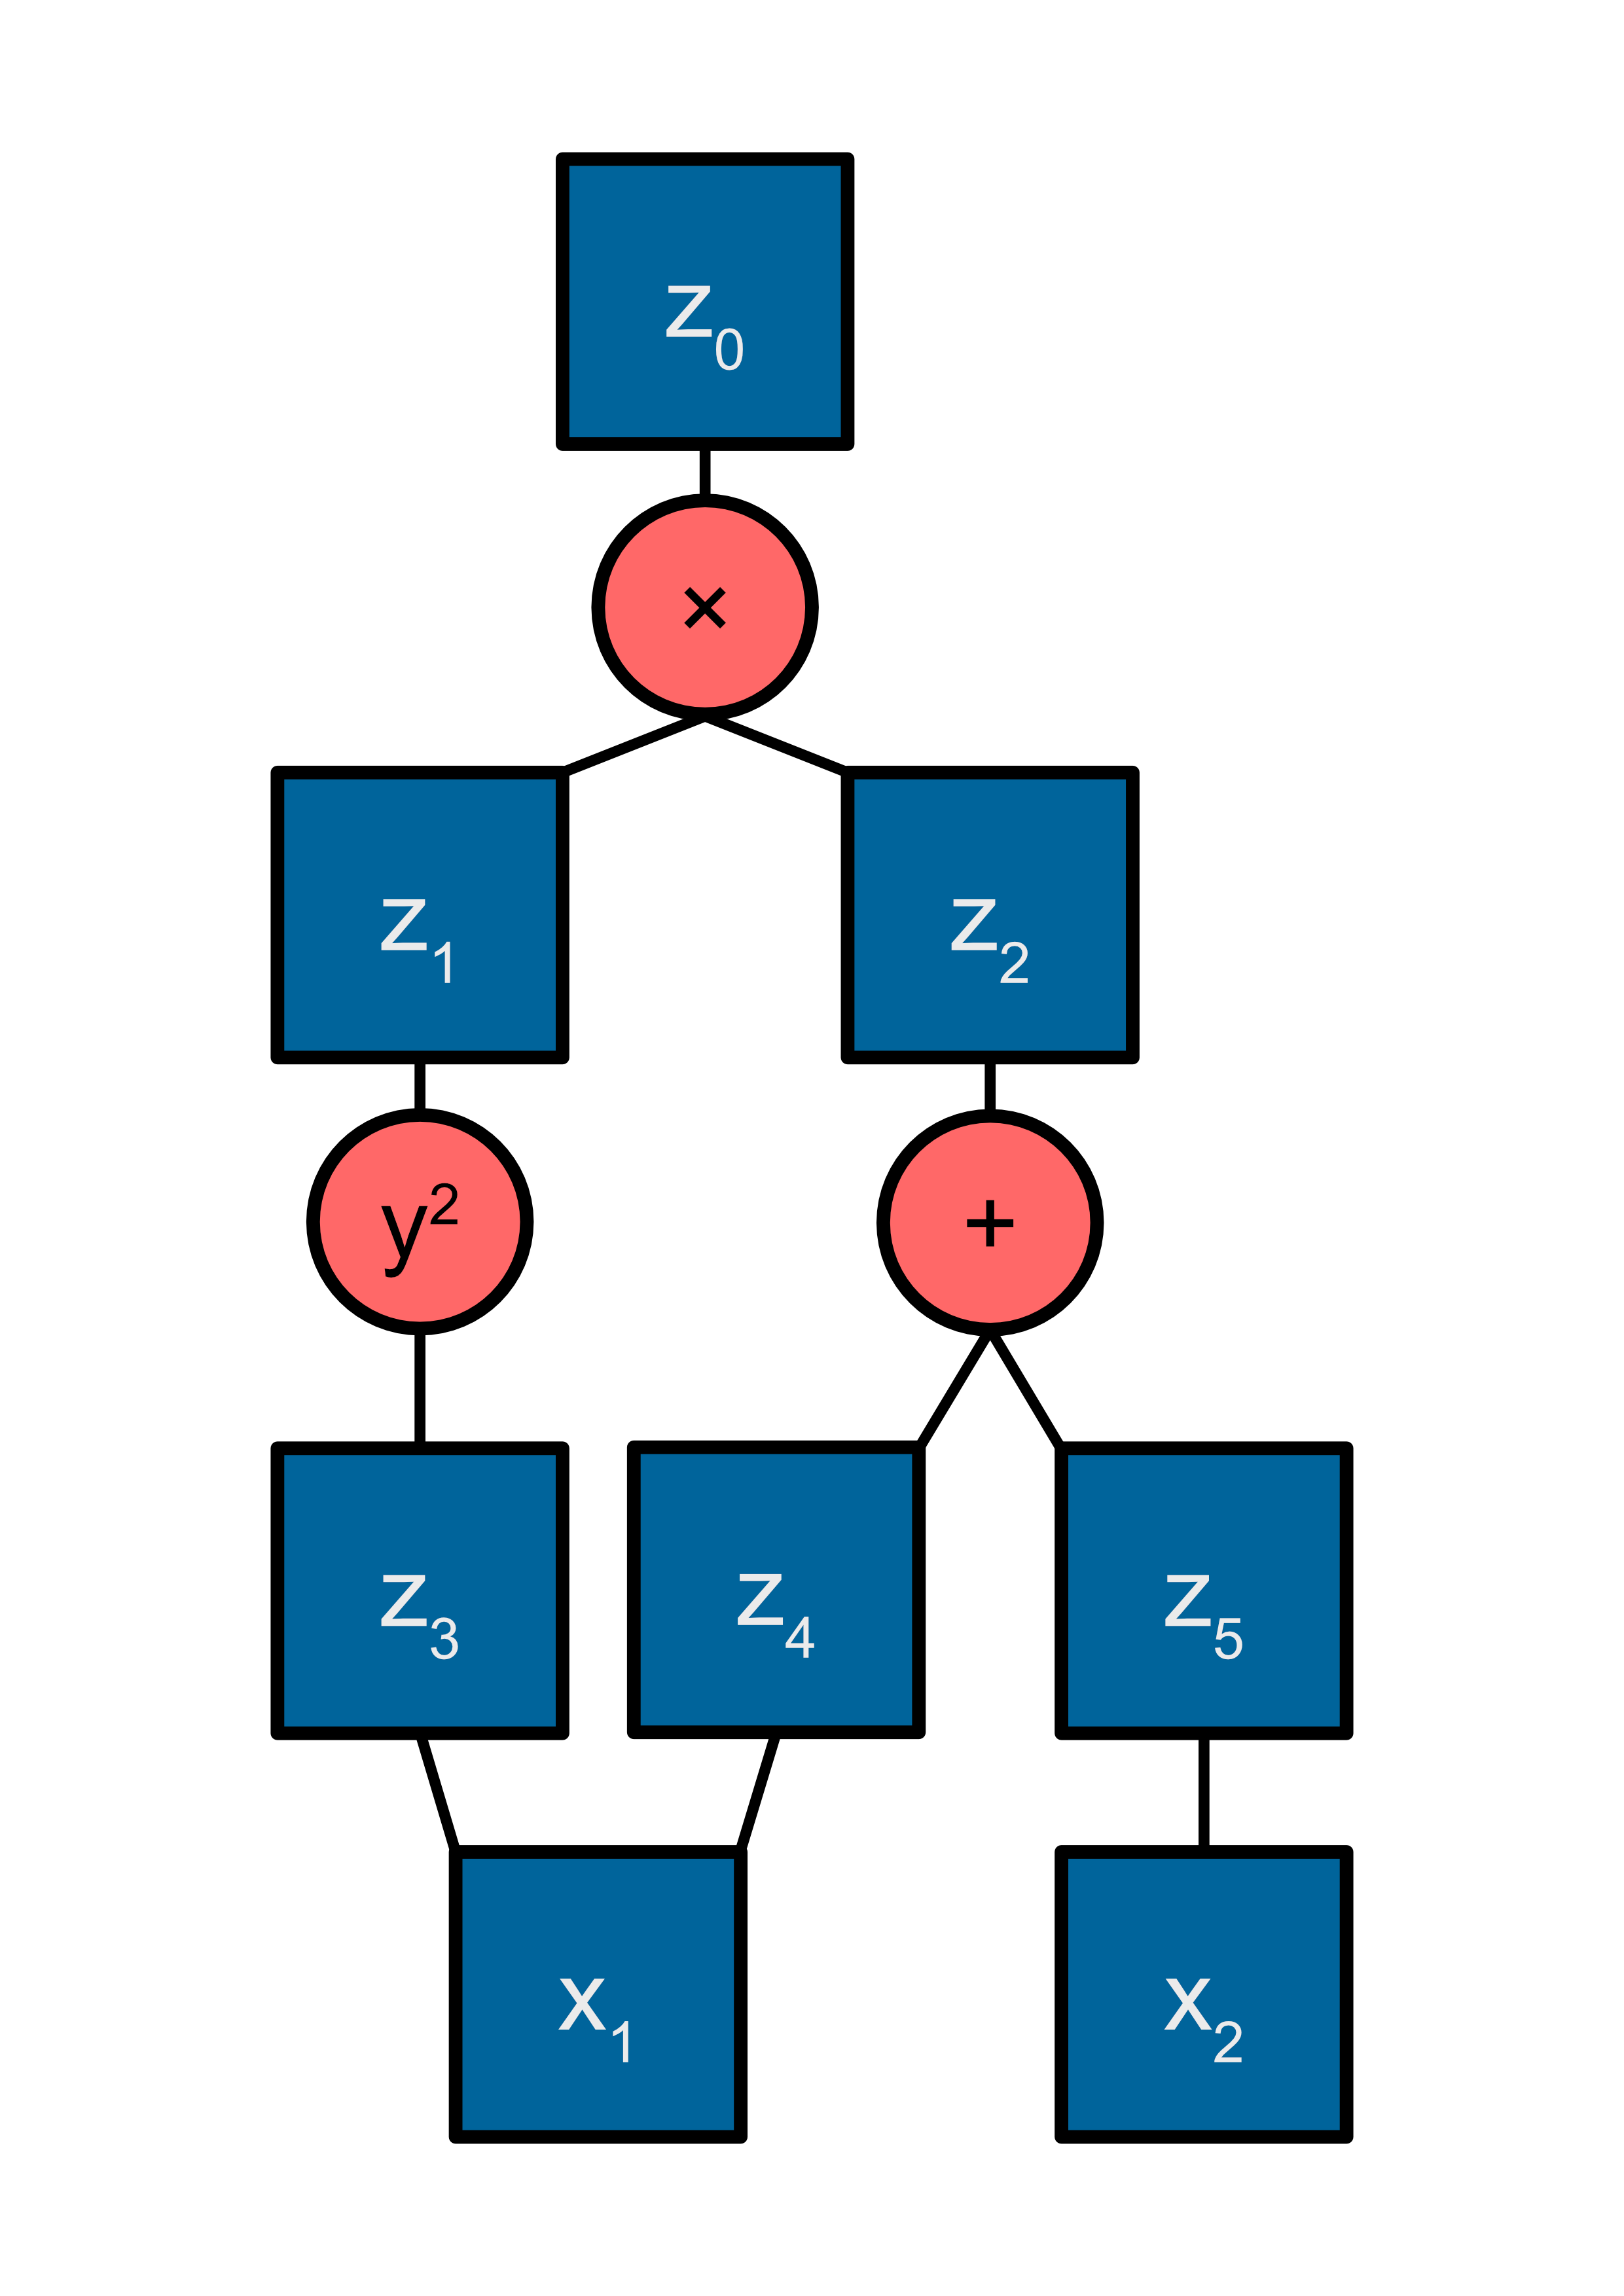
\includegraphics{graph}
    \caption{Tree graph for function $f$ in \refeq{example}.}
    \labfig{tree_graph}
\end{marginfigure}
Then the chain rule is employed which states that
\begin{align}
    (f \circ g (x))' & = f' \circ g(x) \cdot g'(x) \\
    \text{or} \nonumber\\
    \frac{\partial f}{\partial x} & = \frac{\partial f}{\partial g} \frac{\partial g}{\partial x}
    \labeq{chain}
\end{align}

By leveraging \refeq{chain} a function like 
\begin{align}
    f(x_1, x_2) = x_1^2 \cdot (x_1 + x_2)
    \labeq{example}
\end{align}
can be split into smaller pieces
\begin{equation*}
\begin{aligned}[c]
    f(x_1, x_2) & = z_0(x_1, x_2) \\
    z_0(x_1, x_2) & = z_1(x_1, x_2) \cdot z_2(x_1, x_2) \\
    z_1(x_1, x_2) & = (z_3(x_1, x_2))^2 \\
    z_2(x_1, x_2) & = z_4(x_1, x_2) + z_5(x_1, x_2)
\end{aligned}
\qquad
\begin{aligned}[c]
    z_3(x_1, x_2) & = x_1 \\
    z_4(x_1, x_2) & = x_1 \\
    z_5(x_1, x_2) & = x_2
\end{aligned}
\end{equation*}
Each function $z_i$ now involves only a single operation with either one or two inputs.
This makes differentiating $z_i$ with respect to its child node(s) very easy.
\marginnote{The term child node is used since each node $z_i$ (rectangluar shape) is made up of lower level child nodes which are connected via an operation (circular shape).}
\eg
\begin{align}
    \frac{\partial z_1}{\partial z_3} & = 2 z_3
\end{align}
The result of $f$ can now be calculated by inserting some values for the end nodes $x_1$ and $x_2$ and then moving through the tree, from the bottom to the top.
This is called a \textbf{forward pass} as this is also how such equations are solved normally.
At the end, each node is now assigned a value as the forward comes through. \\
Now, how can the gradient of $f$ with respect to the end nodes be obtained? \\
By using the chain rule and walking the graph backwards (hence \textit{back}propagation), the gradients of $f$ with respect to each node can be calculated.
The very first node to start with would be the top-most node $z_0$ which is identical to $f$.
Thus,  $\frac{\partial f}{\partial z_0} = 1$, can be easily obtained.
Calculating the gradient for $z_0$'s child nodes is almost equally easy as the chain rule is applied.
\begin{align}
    \frac{\partial f}{\partial z_1} & = \frac{\partial f}{\partial z_0} \cdot \frac{\partial z_0}{\partial z_1} = 1 \cdot z_2 = z_2 \\
    \frac{\partial f}{\partial z_2} & = \frac{\partial f}{\partial z_0} \cdot \frac{\partial z_0}{\partial z_2} = 1 \cdot z_1 = z_1
\end{align}
So now the gradient for nodes $z_1$ and $z_2$ is known as well.
Notably, the gradients of $z_1$ depends on $z_2$ and vice versa.
This is not a problem, as the gradient is not calculated in the variable node, but in the operator node, which knows all three values $z_0, z_1, z_2$ from the forward-pass.
These calculated gradients are then forwarded to their respective nodes and the process start again.\\
This way gradients for all nodes a propagated (hence back\textit{propagation}) until they reach the end nodes.
As these gradients $\frac{\partial f}{\partial x_1}$ and $\frac{\partial f}{\partial x_2}$ are those which were sought originally, backprop is complete.
\begin{align}
    \frac{\partial f}{\partial x_1} & = \frac{\partial f}{\partial z_3} \cdot \frac{\partial z_3}{\partial x_1} + \frac{\partial f}{\partial z_4} \cdot \frac{\partial z_4}{\partial x_1} \\
    & = 2 z_2 z_3 \cdot 1 + z_1 \cdot 1 = 2 z_2 z_3 + z_1 \\
    \frac{\partial f}{\partial x_2} & = \frac{\partial f}{\partial z_5} \cdot \frac{\partial z_5}{\partial x_2} = z_1 \cdot 1 = z_1 \\
\end{align}
In case of neural networks the end nodes are weights, parameters and inputs.
Most often just the weight gradients are of interest, as the data set or \textit{fixed} parameters should not change.

Interestingly, such a structure assigns each operation a second meaning besides its impact on the forward-pass result.
Each operator now alters the gradient during the backwards-pass as well.
The plus operator as an example just distributes the gradient unaltered to its child nodes.
On the other hand, the gradient is scaled when it passes a multiplication operation. \\
One important fact must be stretched, though:
If the gradient becomes zero, all gradient that come after that node will also be zero!

\section{Vanishing Gradients}
As the previous sectioned ended, shall this section evaluate a little bit further.

Vanishing gradients are a problem that especially deep networks with many weights and many operations have to deal with.
If any weight in a multiplication operation were to become zero is kills the gradient for subsequent operations along the backpropagation.
Subsequently, the very first layers, close to the input, are likely to be subject to smaller gradients than the last few layers, which are very close to the loss function.
Yet, as this is almost unavoidable, other causes for vanishing gradients are.

\subsection{Activation Functions}
Activation functions are often a cause of vanishing gradients.
The first examples of the McCulloch-Pitts neuron and the perceptron used a step-function as activation/classification function.
Looking at the \textbf{step function}, the gradient is zero everywhere except at $x = 0$ where the gradient is infinity.
Such an activation function is obviously of no use and thus not found in any neural network.

Another favorite activation function for nature inspired neural networks are \textbf{sigmoid functions} (logistic function and hyperbolic tangent function).
These seem to not suffer from the same problems, yet in their limit $|x| \rightarrow \inf$ these functions become constant and thus the gradient becomes zero.

\textbf{Rectified Linear Units (ReLU)} were already presented in the previous chapter and their advantage is that they are very easy to compute.
Also, for $x > 0$ ReLU behaves like linear function and just passes the gradient on.
For $x \leq 0$, though, the gradient is sadly zero.

\textbf{Leaky rectifies linear units (leaky ReLU)} do not suffer from this problem.
They do not compare the linear value against $0$ but against the same attenuated linear function.
\begin{align}
    \text{leakyReLU}(x) = \max(\alpha x, x) \text{ with } 0 < \alpha < 1
\end{align}
Leaky ReLU is still easy to compute and thus a popular choice in neural networks.

\subsection{Normalization}
Another way of avoiding vanishing gradients is \textbf{normalization} often just called norm.
Normalization shifts and scales activations such that they represent a normal distribution with $\mu$ and $\sigma$.
$\mu$ and $\sigma$ are both trainable parameters, also called \textbf{affine parameters}.
By doing so, the activations typically are very similar distributed across layers and there are fewer activations with very large amplitudes.
Having well distributed amplitudes helps to avoid gradients exploding or vanishing gradients.

The most common types of normalization are \textbf{batch norm} and \textbf{instance norm}.
Instance norm takes activations for each sample in each channel in a layer and applies normalization over this set~\cite{IN}.\\
Batch norm normalizes over the channel \textit{and} the mini-batch to obtain broader statistics~\cite{BN}.

\subsection{Residual Networks}
Residual networks are another take on tackling the vanishing gradient problem in very deep neural networks 
They introduce skip connections, which forward the signal of a layer add it to the activations of a different layer down the line.
This way the gradients get also forwarded during backprop and maintain their amplitude~\cite{resnet}.
